% Created 2023-10-10 Tue 19:41
% Intended LaTeX compiler: pdflatex
\documentclass[11pt]{article}
\usepackage[utf8]{inputenc}
\usepackage[T1]{fontenc}
\usepackage{graphicx}
\usepackage{longtable}
\usepackage{wrapfig}
\usepackage{rotating}
\usepackage[normalem]{ulem}
\usepackage{amsmath}
\usepackage{amssymb}
\usepackage{capt-of}
\usepackage{hyperref}
\usepackage[margin=0.5in]{geometry}
\author{Bryce Mazurowski}
\date{\today}
\title{1st Assignment - Intro to Parallel Computing}
\hypersetup{
 pdfauthor={Bryce Mazurowski},
 pdftitle={1st Assignment - Intro to Parallel Computing},
 pdfkeywords={},
 pdfsubject={},
 pdfcreator={Emacs 29.1 (Org mode 9.6.6)}, 
 pdflang={English}}
\begin{document}

\maketitle
NCSA Advanced Parallel Computing Cohort
Fall 2023

Due date: October 11, 2023


\section{Describe the two pure ways of parallelism (data and task). Which one of them has the most capability to speed up computationally intensive workloads?}
\label{sec:org6c539b4}
\begin{itemize}
\item Data Parallelism: When a single task is executed on a chunk of data
that is split into pieces based on the number of threads available
for the task
\item Task Parallelism: When multiple independent tasks are executed on a single data
source. Each task can be assigned a thread and computed
concurrently.
\item In general, data parallelism is more capable of speeding up
computationally intensive workflows. When working with a large
dataset, it is quicker to partition the data and work on a given
task concurrently. Task parallelism is also more limited if one task
depends on the operations in a different task.
\end{itemize}

\section{What do you perceive as the best advantage of OpenMP? What is its main limitation?}
\label{sec:org04a770a}
The biggest advantage of OpenMP is its widespread availability. It can
be used on any operating system with basically any compiler. The fact
that it is simple to work with is a close second.

OpenMP's biggest limitation is that it is only effective on shared
memory machines. It cannot handle communication on distributed memory systems.



\section{Write/find a simple serial program with a loop (ask ChatGPT if you can’t find one).}
\label{sec:org76a3c0f}
\begin{enumerate}
\item Parallelize the loop using OpenMP directives
\item Measure the time it takes to complete the loop with a different number of OpenMP threads (1 to 16 suggested)
\item Repeat b) 3-6 times, take the averages, and calculate the speedup factor for each number of threads
\item Plot your results
\item Discuss the scalability of your parallelization. Is it far from ideal? Why?
\end{enumerate}
\subsection{Code}
\label{sec:orgbe6e9e1}
The code takes a vector of complex numbers and computes the number of
iterations for the Mandelbrot set.
\[
f(z) = z^2 + c
\]
where \(z\) and \(c\) are complex numbers. \(z\) is initialized to zero and
the components of \(c\) are randomly generated.

\subsubsection{Serial}
\label{sec:org29fdb15}
\begin{verbatim}
#include <iostream>
#include <vector>
#include <complex>
#include <sys/time.h>

#define ORD 1 << 27

using std::cout;
using std::endl;

typedef std::complex<float> cFloat;

int mandelbrot(cFloat& c);

int main() {
  // instantiate vector of
  std::vector<cFloat> v;
  float a, b;
  srand(time(NULL));
  for (int iPos = 0; iPos < ORD; iPos++) {
    // make 2 random doubles
    a = rand() % RAND_MAX;
    a = float(a) / (RAND_MAX);
    b = rand() % RAND_MAX;
    b = float(b) / (RAND_MAX);
    // make our complex number
    cFloat z(a, b);
    // add it to the vector
    v.push_back(z);
  }

  // stopwatch variables
  struct timeval startTime, stopTime, elapsedTime;

  // now call saxpy
  gettimeofday(&startTime, NULL);
  std::vector<cFloat>::iterator vPos = v.begin();
  std::vector<cFloat>::iterator vEnd = v.end();
  for (; vPos != vEnd; vPos++) {
    std::cout << "vPos = " << (*vPos) << std::endl;
    // calculate setVal
    const int iTs = mandelbrot(*vPos);
    std::cout << "iTs = " << iTs << std::endl;
  }

  gettimeofday(&stopTime, NULL);

  timersub(&stopTime, &startTime, &elapsedTime);
  cout << "Number of args: " << v.size() << "Elapsed time (s): "
       << elapsedTime.tv_sec + elapsedTime.tv_usec / 1000000.0 << endl;

  return 0;
}

int mandelbrot(cFloat &c) {
  cFloat z(0.0, 0.0);
  const unsigned int maxIt = 200;
  for (unsigned int iMan = 0; iMan < maxIt; iMan++) {
    if (std::abs(z) > 2.0) {
      // outside of magnitude bounds
      return iMan;
    }
    // square z
    z = z * z + c;
  }
  return maxIt;
}
\end{verbatim}


\subsubsection{Parallel}
\label{sec:org8174ce6}
\begin{verbatim}
#include <iostream>
#include <vector>
#include <complex>
#include <sys/time.h>
#include "omp.h"

using std::cout;
using std::endl;

typedef std::complex<float> cFloat;

int mandelbrot(cFloat& c);

int main(int argc, char* argv[]) {
  int ORD = 1 << 10;
  if (argc != 1) {
    // ran with 1 << 20
    ORD = 1 << std::stoi(argv[1]);
  }	
  // instantiate vector of complex numbers
  std::vector<cFloat> v;
  float a, b;
  srand(time(NULL));
  for (int iPos = 0; iPos < ORD; iPos++) {
    // make 2 random doubles
    a = rand() % RAND_MAX;
    a = float(a) / (RAND_MAX);
    b = rand() % RAND_MAX;
    b = float(b) / (RAND_MAX);
    // make our complex number
    cFloat z(a, b);
    // add it to the vector
    v.push_back(z);
  }

  // stopwatch variables
  struct timeval startTime, stopTime, elapsedTime;

  gettimeofday(&startTime, NULL);
  // note: must initialize iterator in loop
  // or code segFaults
  #pragma omp parallel
  {
    #pragma omp for
    for (std::vector<cFloat>::iterator vPos = v.begin(); vPos < v.end(); ++vPos) {
      // calculate setVal
      const int iTs = mandelbrot(*vPos);
    }
  }

  gettimeofday(&stopTime, NULL);

  timersub(&stopTime, &startTime, &elapsedTime);
  cout << "Number of args: " << v.size() << " Elapsed time (s): "
       << elapsedTime.tv_sec + elapsedTime.tv_usec / 1000000.0 << endl;

  return 0;
}

int mandelbrot(cFloat &c) {
  cFloat z(0.0, 0.0);
  const unsigned int maxIt = 200;
  for (unsigned int iMan = 0; iMan < maxIt; iMan++) {
    if (std::abs(z) > 2.0) {
      // outside of magnitude bounds
      return iMan;
    }
    // square z
    z = z * z + c;
  }
  return maxIt;
}
\end{verbatim}

\subsection{Results}
\label{sec:org19693de}
Run on a vector of 1048576 complex numbers.
\begin{table}[htbp]
\label{tab:orgc21d5b7}
\centering
\begin{tabular}{rrrrrrrr}
threads & run1 & run2 & run3 & run4 & run5 & avg & speedup\\[0pt]
\hline
1 & 4.27445 & 4.30016 & 4.28323 & 4.26816 & 4.26952 & 4.279104 & 1.\\[0pt]
2 & 2.14344 & 2.17865 & 2.15289 & 2.1612 & 2.14505 & 2.156246 & 1.9845157\\[0pt]
4 & 1.08021 & 1.08807 & 1.08875 & 1.09224 & 1.09027 & 1.087908 & 3.9333326\\[0pt]
8 & 0.57001 & 0.566089 & 0.564286 & 0.564507 & 0.56827 & 0.5666324 & 7.5518167\\[0pt]
16 & 0.31242 & 0.337258 & 0.361114 & 0.300969 & 0.32295 & 0.3269422 & 13.088258\\[0pt]
\end{tabular}
\end{table}
\begin{center}
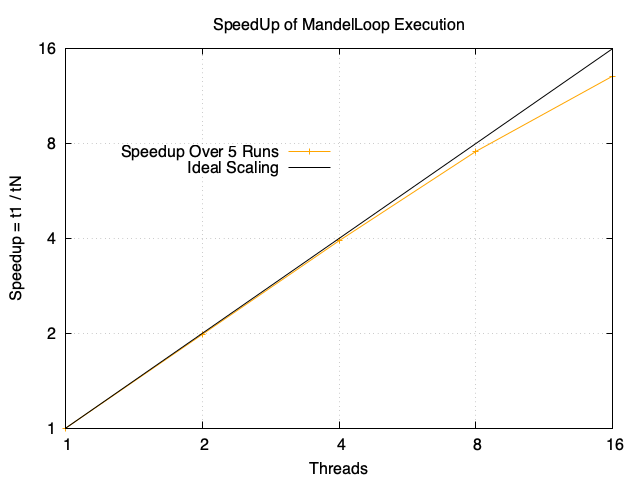
\includegraphics[width=.9\linewidth]{MandelLoop_SpeedUp.png}
\end{center}


The speedup of the program is pretty good. Even with 16 threads it is
close to ideal. Although 8 is maybe a better ideal number of
threads. This may scale even better with a larger vector, but when I
tried the cluster booted me because it took too long with 1 thread.

I think it works well because the task is pretty intensive, sometimes
taking 200 iterations for a single input. In serial we have to wait
for the that to finish. In parallel we get to work while that happens.

One reason it may not be ideal at higher thread counts is that I am
not initializing the vector of complex variables in parallel. This
takes time especially for a vector with over a million
components. That time is effectively constant for all of the thread
counts, and as the time for the Mandelbrot iteration calc goes down it
becomes a more significant portion of the execute time.
\end{document}